\documentclass[12pt,a4paper]{article}
\usepackage{longtable}
\usepackage[LGR,T1]{fontenc}
\usepackage{lscape}
%\usepackage{pdfsync}
\usepackage{multirow}
\usepackage{fancyhdr}
\usepackage{graphicx}
\usepackage{caption}
\usepackage{lastpage}
\usepackage{afterpage}
\usepackage{lettrine}
\usepackage{color,soul}
\usepackage[svgnames]{xcolor}
\usepackage{colortbl}
\usepackage[shortlabels]{enumitem}
\usepackage{tikz}
\usepackage{titlesec}
\usepackage{eurosym}
\usepackage{amsthm}
\usepackage{amsmath}
\usepackage{amssymb}
\usepackage{xr}

\usepackage[round]{natbib}
\bibliographystyle{aer}
\usepackage{booktabs}
\usepackage{threeparttable}

%Palatino font
%\usepackage{pxfonts}
%\usepackage{libertine}
\usepackage[scaled=0.88]{beraserif}
\usepackage[scaled=0.85]{berasans}
\usepackage[scaled=0.84]{beramono}
\usepackage{mathpazo}
%\linespread{1.05}
\usepackage[T1,small,euler-digits]{eulervm}

\usepackage[nomessages]{fp}


 \definecolor{bleuUCLclair}{rgb}{.09, 0.569, 1}
\definecolor{bleuUCLfonce}{rgb}{ .13, .52, .86}
\definecolor{redBurn}{rgb}{.91, 0.29, 0.08}
\definecolor{webbrown}{rgb}{.6,0,0}

\usepackage{hyperref}
\hypersetup{breaklinks = true,  
colorlinks=true, anchorcolor= webbrown, citecolor= webbrown,
filecolor= webbrown, linkcolor= webbrown, menucolor= webbrown,
urlcolor= webbrown, citebordercolor= 1 0 0, menubordercolor=1 0
0, urlbordercolor=1 0 0, runbordercolor=1 0 0 }
\addtolength{\topmargin}{-1.5cm}
\addtolength{\textheight}{1.5cm}
\addtolength{\textwidth}{2cm}
\addtolength{\footskip}{2cm}
\setlength{\evensidemargin}{-0.5cm}
\setlength{\oddsidemargin}{-0.5cm}
\setlength{\arrayrulewidth}{0.25pt}

\renewcommand{\baselinestretch}{1.1} % Interligne


\newenvironment{maliste}%
{ \begin{list}%
	{\textcolor{bleuUCLfonce}{$\bullet$}\hspace{0.5cm}}%
	{\setlength{\labelwidth}{50pt}%
	 \setlength{\leftmargin}{25pt}%
	 \setlength{\itemsep}{30pt}}}%
{ \end{list} }

%\renewcommand{\headrulewidth}{0.0pt}
%\newcommand{\clearemptydoublepage}{%
%	\newpage{\pagestyle{empty}\cleardoublepage}}

% qting package loaded later with external documents
% \usepackage{../../../utils/styles/qting}
% \quotefrom{../../../paper/sections/intro.tex}
% \quotefrom{../../../paper/sections/analytic.tex}

%section like title in longtable
\newcommand{\seclong}[1]{\multicolumn{2}{@{}l}{{\Large\sffamily #1}} 
\vspace{0.5cm}
\\}

%enumerate on two columns
\newcounter{listlong}
\newcommand{\newlistlong}{\setcounter{listlong}{1}}
\newcommand{\iteml}[1]{%
\hspace{4.5cm}\textcolor{redBurn}{\arabic{listlong}}\stepcounter{listlong}%
&%
#1%
 
\\%
}

%left in column
\newcommand{\lcol}[1]{%
\begin{minipage}[t]{.35\textwidth}%

#1%

\end{minipage}%
}

\title{\vspace{-1cm}
\begin{flushleft} {\sffamily \emph{Paper title}: reply to reviewers }\end{flushleft}}
\date{\vspace{-1.7cm}\begin{flushleft}\sffamily Paper authors\end{flushleft}}


\pagestyle{fancy} 
\fancyhf{}
\fancyfoot[R]{\sffamily\thepage\ / \pageref{LastPage}}
  \fancyfoot[L]{ }

\fancypagestyle{plain}{%
  \fancyhf{}%
  \fancyfoot[R]{\sffamily\thepage\ / \pageref{LastPage}}
  \fancyfoot[L]{ }
}

\renewcommand{\headrulewidth}{0.0pt}


\newcommand{\hlc}[2][yellow]{ {\sethlcolor{#1} \hl{$^{TODO:}$#2}} }

\newcommand{\paolo}[2][green]{ {\sethlcolor{#1} \hl{$^{P:}$#2}} }


\titleformat{\section}
{\bfseries\scshape}{Reviewer \# \thesection}{1em}{}

\titleformat{\subsection}
{\normalfont\scshape}{Comment \# \thesubsection}{1em}{}

\usepackage[framemethod=default]{mdframed}
%\mdfsetup{skipabove=\topskip,skipbelow=\topskip}

\global\mdfdefinestyle{comment}{%
     linecolor=Crimson!50,linewidth=0.1cm,backgroundcolor=Crimson!5,%
     leftmargin=-0.5cm,rightmargin=-0.5cm, innerleftmargin=0.4cm,innerrightmargin=0.4cm,
     topline=false,bottomline=false
}

\global\mdfdefinestyle{commentbox}{%
     linecolor=Crimson!50,linewidth=0.1cm,backgroundcolor=Crimson!5,%
     leftmargin=-0.5cm,rightmargin=-0.5cm, innerleftmargin=0.4cm,innerrightmargin=0.4cm,
     topline=false,bottomline=false
}

\global\mdfdefinestyle{manuscript}{%
     linecolor=gray!10,linewidth=0.05cm,backgroundcolor=gray!10,%
     leftmargin=-0.5cm,rightmargin=-0.5cm, innerleftmargin=0.4cm,innerrightmargin=0.4cm
}
  
  \renewcommand{\subsectionautorefname}{Comment}
  
\newcommand{\comment}[1]{\subsection{}
\begin{mdframed}[style=comment] 
		\textit{#1}
\end{mdframed}}

\newcommand{\commentbox}[1]{
\begin{mdframed}[style=commentbox] 
		\textit{#1}
\end{mdframed}}



\newcommand{\reply}[1]{
	\noindent\textbf{Reply:}

\noindent #1
\\
}

\newcommand{\changes}[1]{
	\noindent\textbf{Changes:}
	\vspace{-5pt}
\begin{mdframed}[style=manuscript] 
	#1
\end{mdframed}}

\newcommand{\changesbox}[1]{
	\noindent\vspace{-8pt}
\begin{mdframed}[style=manuscript] 
	#1
\end{mdframed}}

%DIF PREAMBLE EXTENSION ADDED BY LATEXDIFF
%DIF UNDERLINE PREAMBLE %DIF PREAMBLE
\RequirePackage[normalem]{ulem} %DIF PREAMBLE
\RequirePackage{color}\definecolor{RED}{rgb}{1,0,0}\definecolor{BLUE}{rgb}{0,0,1} %DIF PREAMBLE
\providecommand{\DIFaddtex}[1]{{\protect\color{blue}\uwave{#1}}} %DIF PREAMBLE
\providecommand{\DIFdeltex}[1]{{\protect\color{red}\sout{#1}}}                      %DIF PREAMBLE
%DIF SAFE PREAMBLE %DIF PREAMBLE
\providecommand{\DIFaddbegin}{} %DIF PREAMBLE
\providecommand{\DIFaddend}{} %DIF PREAMBLE
\providecommand{\DIFdelbegin}{} %DIF PREAMBLE
\providecommand{\DIFdelend}{} %DIF PREAMBLE
\providecommand{\DIFmodbegin}{} %DIF PREAMBLE
\providecommand{\DIFmodend}{} %DIF PREAMBLE
%DIF FLOATSAFE PREAMBLE %DIF PREAMBLE
\providecommand{\DIFaddFL}[1]{\DIFadd{#1}} %DIF PREAMBLE
\providecommand{\DIFdelFL}[1]{\DIFdel{#1}} %DIF PREAMBLE
\providecommand{\DIFaddbeginFL}{} %DIF PREAMBLE
\providecommand{\DIFaddendFL}{} %DIF PREAMBLE
\providecommand{\DIFdelbeginFL}{} %DIF PREAMBLE
\providecommand{\DIFdelendFL}{} %DIF PREAMBLE
%DIF HYPERREF PREAMBLE %DIF PREAMBLE
\providecommand{\DIFadd}[1]{\texorpdfstring{\DIFaddtex{#1}}{#1}} %DIF PREAMBLE
\providecommand{\DIFdel}[1]{\texorpdfstring{\DIFdeltex{#1}}{}} %DIF PREAMBLE
\newcommand{\DIFscaledelfig}{0.5}
%DIF HIGHLIGHTGRAPHICS PREAMBLE %DIF PREAMBLE
\RequirePackage{settobox} %DIF PREAMBLE
\RequirePackage{letltxmacro} %DIF PREAMBLE
\newsavebox{\DIFdelgraphicsbox} %DIF PREAMBLE
\newlength{\DIFdelgraphicswidth} %DIF PREAMBLE
\newlength{\DIFdelgraphicsheight} %DIF PREAMBLE
% store original definition of \includegraphics %DIF PREAMBLE
\LetLtxMacro{\DIFOincludegraphics}{\includegraphics} %DIF PREAMBLE
\newcommand{\DIFaddincludegraphics}[2][]{{\color{blue}\fbox{\DIFOincludegraphics[#1]{#2}}}} %DIF PREAMBLE
\newcommand{\DIFdelincludegraphics}[2][]{% %DIF PREAMBLE
	\sbox{\DIFdelgraphicsbox}{\DIFOincludegraphics[#1]{#2}}% %DIF PREAMBLE
	\settoboxwidth{\DIFdelgraphicswidth}{\DIFdelgraphicsbox} %DIF PREAMBLE
	\settoboxtotalheight{\DIFdelgraphicsheight}{\DIFdelgraphicsbox} %DIF PREAMBLE
	\scalebox{\DIFscaledelfig}{% %DIF PREAMBLE
		\parbox[b]{\DIFdelgraphicswidth}{\usebox{\DIFdelgraphicsbox}\\[-\baselineskip] \rule{\DIFdelgraphicswidth}{0em}}\llap{\resizebox{\DIFdelgraphicswidth}{\DIFdelgraphicsheight}{% %DIF PREAMBLE
				\setlength{\unitlength}{\DIFdelgraphicswidth}% %DIF PREAMBLE
				\begin{picture}(1,1)% %DIF PREAMBLE
					\thicklines\linethickness{2pt} %DIF PREAMBLE
					{\color[rgb]{1,0,0}\put(0,0){\framebox(1,1){}}}% %DIF PREAMBLE
					{\color[rgb]{1,0,0}\put(0,0){\line( 1,1){1}}}% %DIF PREAMBLE
					{\color[rgb]{1,0,0}\put(0,1){\line(1,-1){1}}}% %DIF PREAMBLE
				\end{picture}% %DIF PREAMBLE
			}\hspace*{3pt}}} %DIF PREAMBLE
} %DIF PREAMBLE
\LetLtxMacro{\DIFOaddbegin}{\DIFaddbegin} %DIF PREAMBLE
\LetLtxMacro{\DIFOaddend}{\DIFaddend} %DIF PREAMBLE
\LetLtxMacro{\DIFOdelbegin}{\DIFdelbegin} %DIF PREAMBLE
\LetLtxMacro{\DIFOdelend}{\DIFdelend} %DIF PREAMBLE
\DeclareRobustCommand{\DIFaddbegin}{\DIFOaddbegin \let\includegraphics\DIFaddincludegraphics} %DIF PREAMBLE
\DeclareRobustCommand{\DIFaddend}{\DIFOaddend \let\includegraphics\DIFOincludegraphics} %DIF PREAMBLE
\DeclareRobustCommand{\DIFdelbegin}{\DIFOdelbegin \let\includegraphics\DIFdelincludegraphics} %DIF PREAMBLE
\DeclareRobustCommand{\DIFdelend}{\DIFOaddend \let\includegraphics\DIFOincludegraphics} %DIF PREAMBLE
\LetLtxMacro{\DIFOaddbeginFL}{\DIFaddbeginFL} %DIF PREAMBLE
\LetLtxMacro{\DIFOaddendFL}{\DIFaddendFL} %DIF PREAMBLE
\LetLtxMacro{\DIFOdelbeginFL}{\DIFdelbeginFL} %DIF PREAMBLE
\LetLtxMacro{\DIFOdelendFL}{\DIFdelendFL} %DIF PREAMBLE
\DeclareRobustCommand{\DIFaddbeginFL}{\DIFOaddbeginFL \let\includegraphics\DIFaddincludegraphics} %DIF PREAMBLE
\DeclareRobustCommand{\DIFaddendFL}{\DIFOaddendFL \let\includegraphics\DIFOincludegraphics} %DIF PREAMBLE
\DeclareRobustCommand{\DIFdelbeginFL}{\DIFOdelbeginFL \let\includegraphics\DIFdelincludegraphics} %DIF PREAMBLE
\DeclareRobustCommand{\DIFdelendFL}{\DIFOaddendFL \let\includegraphics\DIFOincludegraphics} %DIF PREAMBLE
%DIF LISTINGS PREAMBLE %DIF PREAMBLE
\RequirePackage{listings} %DIF PREAMBLE
\RequirePackage{color} %DIF PREAMBLE
\lstdefinelanguage{DIFcode}{ %DIF PREAMBLE
	%DIF DIFCODE_UNDERLINE %DIF PREAMBLE
	moredelim=[il][\color{red}\sout]{\%DIF\ <\ }, %DIF PREAMBLE
	moredelim=[il][\color{blue}\uwave]{\%DIF\ >\ } %DIF PREAMBLE
} %DIF PREAMBLE
\lstdefinestyle{DIFverbatimstyle}{ %DIF PREAMBLE
	language=DIFcode, %DIF PREAMBLE
	basicstyle=\ttfamily, %DIF PREAMBLE
	columns=fullflexible, %DIF PREAMBLE
	keepspaces=true %DIF PREAMBLE
} %DIF PREAMBLE
\lstnewenvironment{DIFverbatim}{\lstset{style=DIFverbatimstyle}}{} %DIF PREAMBLE
\lstnewenvironment{DIFverbatim*}{\lstset{style=DIFverbatimstyle,showspaces=true}}{} %DIF PREAMBLE
%DIF END PREAMBLE EXTENSION ADDED BY LATEXDIFF

%----Helper code for dealing with external references----
% (by cyberSingularity at http://tex.stackexchange.com/a/69832/226)


\makeatletter

\newcommand*{\addFileDependency}[1]{% argument=file name and extension
\typeout{(#1)}% latexmk will find this if $recorder=0
% however, in that case, it will ignore #1 if it is a .aux or 
% .pdf file etc and it exists! If it doesn't exist, it will appear 
% in the list of dependents regardless)
%
% Write the following if you want it to appear in \listfiles 
% --- although not really necessary and latexmk doesn't use this
%
\@addtofilelist{#1}
%
% latexmk will find this message if #1 doesn't exist (yet)
\IfFileExists{#1}{}{\typeout{No file #1.}}
}\makeatother

\newcommand*{\myexternaldocument}[1]{%
\externaldocument{#1}%
\addFileDependency{#1.tex}%
\addFileDependency{#1.aux}%
}
%------------End of helper code--------------

\usepackage{utils/styles/qting}

% Commands used in quoted content from the paper (defined in BSZ.tex but not loaded here)
\newcommand{\paratitle}[1]{\vspace{1em}\noindent\textbf{#1}\hspace{1ex}}

\myexternaldocument{BSZ.tex}

\quotefrom{BSZ}

\quotefrom{sections/model.tex}

\quotefrom{sections/characterization.tex}

\quotefrom{sections/analytic.tex}

\quotefrom{sections/facts.tex}

\quotefrom{sections/quantitative.tex}

\quotefrom{sections/conclusion.tex}

\usepackage{utils/styles/qting}

% % Commands used in quoted content from the paper (defined in BSZ.tex but not loaded here)
% \newcommand{\paratitle}[1]{\vspace{1em}\noindent\textbf{#1}\hspace{1ex}}

% \myexternaldocument{../../../paper/build/BSZ}

% \quotefrom{../../../paper/BSZ}

% \quotefrom{../../../paper/sections/model.tex}

% \quotefrom{../../../paper/sections/characterization.tex}

% \quotefrom{../../../paper/sections/analytic.tex}


% \quotefrom{../../../paper/sections/facts.tex}

% \quotefrom{../../../paper/sections/quantitative.tex}

% \quotefrom{../../../paper/sections/conclusion.tex}

% Environments  
\newtheorem{lemma}{Lemma}
\newtheorem{proposition}{Proposition}
\newtheorem{theorem}{Theorem}
\newtheorem{claim}[theorem]{Claim}
\newtheorem{corollary}{Corollary}
\newtheorem{definition}{Definition}
\newtheorem{example}{Example}
\newtheorem{assumption}{Assumption}
%\newtheorem{proposition}[theorem]{Proposition}
\newtheorem{remark}{Remark}
\newtheorem{problem}{Problem}

\begin{document}

% \input{Letters/Letters_MainChange.tex}

% \newpage

% \section*{Response to the Editor\bigskip{}
}

Dear Editor,\bigskip{}

Thank you for the opportunity to revise and resubmit our paper. We appreciate the thoughtful comments from the referees and have addressed their concerns in this revision.\medskip{}

% Add your response to the Editor here

%%%% DS: I made changes to the next two paragraphs. Original version below.
We now frame the paper as a frictionless benchmark model in which beliefs serve as a direct source of business cycle fluctuations. 
In this benchmark, there are no financial frictions, no short-selling constraints, prices are fully flexible, and markets are complete. 
Beliefs and output are only linked through a timing assumption: firms must choose labor input before observing their productivity. 
We see value in developing such a frictionless benchmark, as it allows us to isolate the direct effects of beliefs on business cycles. 
These effects are likely to be present-- and potentially be amplified---in environments that feature additional frictions. \medskip{}

% We also invested effort to produce new theoretical insights and provide greater empirical support. 
While your second route suggested we focus on the qualitative properties, we also pursued a quantitative evaluation of the model. 
% Our goal was to show the extent the model can produce quantitatively sensible predictions.  
We purposely avoid introducing many bells and whistles, as we wanted to keep the model parsimonious, introducing only minor changes to facilitate the calibration.
Despite its simplicity, the model produces reasonable predictions for both asset prices and labor market fluctuations. 
Section~\ref{sec:quantitative} now includes a more comprehensive quantitative assessment, which substantially improves upon the earlier version we had presented. \medskip{}


% \newpage

\section*{Response to Referee \#1\bigskip{}
}

Dear Referee,\bigskip{}

Thank you for your comments and suggestions. We have carefully considered your feedback and have revised the paper accordingly.\medskip{}

\subsection*{Major comments I}

\commentbox{
Most important, I think the authors could try and illustrate a little bit more the novel
empirical implications of their model, ideally by comparing the model and the data. In
particular, what empirical implications does your model have that others don't (e.g. using
survey data)? I find the quantitative section a little disappointing in that regard, since you
match mostly standard moments. The facts presented in section 2, while useful, are fairly
well known and general.
\begin{itemize}
    \item One simple implication that comes to mind is that the model predicts that earnings
    (or dividends, in the model) become more volatile when the share of wealth held by optimistic 
    is larger, e.g. when the expansion is longer. 
    Do we have evidence for this? Even something highly stylized would help.
    \item The model is about TFP growth, but some of the empirics use earnings growth, 
    Some of the empirics use dividend growth. Do you think it would make sense to look at TFP
    forecasts (or GDP forecasts perhaps)? These changed a lot over time, for instance
    in the 1990s. There is a literature on how long it takes to learn about TFP shocks; for
    instance, Edge Laubach Williams JME 2007.
    \item     Could we measure the dispersion in beliefs in IBES (or the SPF, or...) and see if the
    dispersion has implications? I guess in the model it has to be wealth-weighted.
    \item Some models that might be natural comparisons are the ones where agents are
    heterogeneous in risk aversion; when beliefs are different but fixed; and when
    there is not full risk sharing between the worker and the entrepreneur (which I
    think can be done relatively easily assuming for instance hand to mouth workers).
    \item I apologize that this comment is a little vague, as I don't have a very clear
    suggestion, but hopefully you understand my desire for more empirical implications.
\end{itemize}
}

We thank you for this thoughtful comment. In the revised version of the paper, we
substantially expanded the discussion of the model's novel empirical implications and
added new theoretical and empirical material to better illustrate what distinguishes
our framework from related models.

\paragraph{1. State-dependent link between belief dispersion and trading volume.}

We focus in particular on your suggestion regarding belief dispersion.
The revised paper develops a new empirical implication of the model:
under rank-alternating beliefs, the relationship between belief dispersion
and trading volume is state-dependent.
Specifically, turnover responds more strongly to disagreement in recessions
than in expansions.

This asymmetry arises from the interaction of two forces in the model:
(i) a rebalancing effect driven by wealth dynamics, and
(ii) a change-in-beliefs effect that operates when agents switch from
optimism to pessimism (or vice versa) across states.
Under rank-alternating beliefs, these forces reinforce each other in downturns
but partially offset each other in expansions, generating a sharp
and testable prediction.

We added a new subsection that formally characterizes this mechanism
and derives closed-form expressions linking turnover to belief dispersion.
The section then takes this prediction to the data.
Using IBES analyst expectations, we construct a measure of aggregate disagreement
that mirrors the model’s structure and estimate time-series regressions
of stock market turnover on this measure.

Consistent with the theory, we find that turnover is significantly more
sensitive to disagreement during recessions,
with the strongest effects occurring at the onset of downturns.
The results are robust to controlling for aggregate volatility (VIX)
and market returns.

To the best of our knowledge, this state-dependent link between belief dispersion
and trading volume has not been documented in the literature and constitutes
a novel empirical implication of our framework.

Section~\ref{sec: trading_volume} of the revised paper provides a detailed
discussion. The first part derives the analytical relationship between turnover
and belief dispersion. The second part implements the empirical test
using IBES and CRSP data.

We reproduce below the theoretical discussion from Section~\ref{sec: trading_volume} of the revised paper.
\changesbox{
    \quoting{TradingVolumeTheory}
}

Next, we reproduce the empirical discussion from Section~\ref{sec: trading_volume} of the revised paper.
\changesbox{
    \quoting{EmpiricalEvidenceI}
    \quoting{EmpiricalEvidenceII}
}

\begin{table}[!t]\centering
    \caption{Turnover Regressions with Standardized Disagreement}
    \label{tab:turnover_di_5specs_standardized_letter}
    
    \resizebox{\textwidth}{!}{%
    \begin{tabular}{lccccc}
    \hline\hline
     & Baseline & Rec $\times$ DI & Rec $\times$ DI 
     & Early Rec. & Early Rec. \\
     & (1) & (2) & (3) & (4) & (5) \\
    \hline
    Disagreement (z-score) 
        & 0.075 & 0.054 & 0.054 & 0.069 & 0.069 \\
        & (0.047) & (0.039) & (0.039) & (0.047) & (0.047) \\
    
    Recession 
        &  & 0.051 &  &  &  \\
        &  & (0.048) &  &  &  \\
    
    Disagreement $\times$ Recession 
        &  & 0.176*** & 0.188*** &  &  \\
        &  & (0.058) & (0.061) &  &  \\
    
    Early Rec. (first 2 qtrs) 
        &  &  &  & 0.014 &  \\
        &  &  &  & (0.035) &  \\
    
    Disagreement $\times$ Early Rec. 
        &  &  &  & 0.095* & 0.098* \\
        &  &  &  & (0.051) & (0.051) \\
    
    \hline
    Marginal effect of DI in recession 
        &  & 0.230 & 0.242 & 0.164 & 0.167 \\
    
    Constant 
        & 0.311*** & 0.301*** & 0.305*** & 0.309*** & 0.309*** \\
        & (0.023) & (0.022) & (0.020) & (0.023) & (0.022) \\
    
    \hline
    Observations & 158 & 158 & 158 & 158 & 158 \\
    $R^2$ & 0.212 & 0.352 & 0.344 & 0.235 & 0.235 \\
    \hline\hline
    \end{tabular}%
    }
    
    \vspace{0.2em}
    {\begin{flushleft}
        \footnotesize
        Sample period: 1982Q2--2021Q3. Disagreement is standardized within sample.
        Newey--West (lag 4) standard errors in parentheses.
        * $p<0.10$, ** $p<0.05$, *** $p<0.01$.
        \end{flushleft}}
    
    
    \end{table}    

\paragraph{2. TFP growth survey expectations.}

You raise the important question of whether the empirical analysis should focus
more directly on expectations of TFP growth, given that the model is formulated
in terms of productivity dynamics.

Direct survey data on TFP growth expectations are unfortunately limited.\footnote{
For instance, \citet{edge2007learning} use expectations about output per worker rather than TFP itself due to data limitations.
}
However, it is possible to construct survey-based proxies for productivity growth
using expectations of GDP and employment growth from the Survey of Professional
Forecasters (SPF).

In the revised paper, we therefore added a new subsection
(Section~\ref{sec:biases_expectations.sec})
that evaluates whether the model can reproduce the empirical properties of
subjective productivity-growth expectations.

Specifically, we estimate Coibion--Gorodnichenko (CG) regressions for two survey-based
productivity measures—labor productivity growth and a TFP proxy—and compare the
forecast-revision coefficient in the data to the corresponding coefficient
obtained from simulated data in the calibrated model.

In the data, the CG coefficient is $-0.63$ for labor productivity
and $-0.50$ for the TFP proxy,
indicating substantial over-extrapolation in productivity expectations.
The calibrated model implies a coefficient of $-0.695$.
This value is quantitatively close to the empirical estimate for labor productivity
and lies within one standard error of the estimate for the TFP proxy.

Importantly, the model was not calibrated to match productivity-expectation moments.
Nevertheless, it reproduces the magnitude of the forecast-bias pattern observed in survey data.
This shows that the belief distortions that generate endogenous movements in
labor demand and risk premia also imply empirically realistic biases
in productivity-growth expectations.

We believe this addition strengthens the paper by linking the model more directly
to survey-based evidence on expectation formation.
We thank you for this suggestion.

We reproduce below the discussion from Section~\ref{sec:biases_expectations.sec} of the revised paper.

\changesbox{
    \quoting{ProdExpectationI}
    \quoting{ProdExpectationII}
}

\begin{table}[!t]
    \centering
    \caption{Coibion--Gorodnichenko Regressions for Productivity Measures}
    \label{tab:cg_productivity_letter}
    \begin{threeparttable}
    \begin{tabular}{lcc}
    \toprule
     & Labor Productivity & TFP Proxy \\
    \midrule
    Forecast revision coefficient $\beta_{CG}$ 
    & -0.63$^{***}$ 
    & -0.50$^{**}$ \\
    & (0.030) & (0.198) \\
    Constant 
    & -0.15 
    & -0.25 \\
    & (0.289) & (0.259) \\
    \midrule
    Observations 
    & 86 & 86 \\
    $R^2$ 
    & 0.3697 & 0.0579 \\
    Adj. $R^2$ 
    & 0.3622 & 0.0467 \\
    % Newey--West lag 
    % & 4 & 4 \\
    Sample 
    & 2004Q1--2025Q2 & 2004Q1--2025Q2 \\
    \bottomrule
    \end{tabular}
    \begin{tablenotes}[flushleft]
    \footnotesize
    \item Notes: Each column reports OLS estimates of
    $\text{FE}_t = c + \beta \,\text{Revision}_t + u_t$, where $h=1$ quarter.
    Reported standard errors (in parentheses) are Newey--West HAC with lag 4.
    Labor productivity uses $\Delta y - \Delta n$.
    TFP proxy uses $\Delta y - \alpha \Delta n$ with $\alpha=2/3$.
    Significance: $^{*} p<0.10$, $^{**} p<0.05$, $^{***} p<0.01$ (based on HAC $p$-values).
    \end{tablenotes}
    \end{threeparttable}
    \end{table}


    \paragraph{3. Volatility amplification and the share of wealth held by optimists.}

    The model also implies that dividend volatility increases when the share of wealth
    held by optimistic investors is larger—for instance, following a prolonged expansion.
    In the revised paper, we clarify this mechanism and make explicit that the amplification
    operates through endogenous labor demand and operating leverage.
    
    The mechanism unfolds in three steps.
    First, when wealth becomes more concentrated in the hands of optimistic investors,
    the overall level of market optimism rises and objective risk premia decline.
    Optimistic investors are more willing to bear risk, which compresses the risk premium,
    as shown in Section~\ref{sec:beliefs_asset_prices_labor_demand.sec}.
    
    Second, lower risk premia increase the present value of future profits and induce firms
    to expand labor demand.
    This raises the labor share of output.
    
    Third, a higher labor share increases operating leverage:
    because labor is chosen in advance and represents a quasi-fixed cost,
    profits (and hence dividends) become more sensitive to productivity shocks.
    As a result, dividend volatility increases when optimism—and therefore labor demand—is high.
    
    Directly measuring wealth-weighted optimism in the data is challenging.
    However, each component of this mechanism is supported by existing empirical evidence.
    First, the link between optimism and lower expected returns is well documented
    (e.g., \citealt{de_la_o_subjective_2021}).
    Second, higher labor share predicts lower expected returns,
    consistent with compressed risk premia (\citealt{santos2006labor}),
    and aggregate hiring rates negatively predict stock returns (\citealt{belo2023drives}),
    consistent with the labor-demand channel.
    Third, \citet{donangelo2019cross} show that the labor share is a proxy for operating leverage
    and that higher labor share is associated with greater sensitivity of profits to shocks.
    
    Taken together, this body of evidence is consistent with the model’s prediction
    that periods of elevated optimism—when wealth is more concentrated among optimists—
    are associated with greater operating leverage and higher dividend volatility.

    We make the connection with the empirical evidence in the discussion of the model's predictions in Section~\ref{sec:analysis.sec4} of the revised paper. 
    The discussion of this mechanism is reproduced below.

    \changesbox{
        \quoting{FrothyMarkets}
    }

\paragraph{4. Distinction from alternative mechanisms.}

Finally, we clarify in the revised draft how our predictions differ from alternative
heterogeneous-agent frameworks.

You mention two natural benchmarks: models with heterogeneous risk aversion, and models where there is not full risk sharing between workers and investors.

Models with heterogeneous risk aversion implies the ranking of investors in terms of risk-taking is fixed: more risk-tolerant agents tend to take more risk.
This property is analogous to the case of rank-preserving beliefs shown in Figure \ref{fig: het_beliefs1}.
Hence, the implications of models with heterogeneous risk aversion should be similar to models with rank-preserving beliefs, and it will be different from models with rank-alternating beliefs.

We discuss this point in more detail in Section~\ref{sec:belief_taxonomy.sec} of the revised paper.

\changesbox{
    \quoting{RiskAversionDiscussion}
}

You also mention models where there is not full risk sharing between workers and investors.
Appendix~\ref{sec: hand_to_mouth_workers} describes a version of the model where labor is supplied by hand-to-mouth workers rather than by investors.
We show that this modification leaves our main results essentially unchanged.
In particular, in the special case of linear labor disutility ($\nu = 0$) considered in Section~\ref{sec:analysis.sec4}, the equilibrium allocation and asset prices are identical to those in the baseline model.

We reproduce below the characterization of the equilibrium in the hand-to-mouth version of the model from Appendix~\ref{sec: hand_to_mouth_workers}.
\changesbox{
    \quoting{HandToMouthWorkers}
}

We refer to this analysis in Section~\ref{sec:analysis.sec4} of the revised paper.
\changesbox{
    \quoting{CiteWorkers}
}


\paragraph{Taking stock.}

In response to your comment, the revised paper now makes explicit several empirical implications of the model that go beyond matching standard asset-pricing moments. In particular, we show that the framework can account for:

\begin{enumerate}
    \item A state-dependent relationship between belief dispersion and trading volume.
    \item The magnitude of forecast biases in productivity-growth expectations, as measured by Coibion--Gorodnichenko regressions.
    \item The joint occurrence of low risk premia and elevated risk exposure during booms.
    \item The link between survey expectations and objective risk premia.
    \item Standard asset-pricing moments, including the level of the equity premium, return volatility, and return predictability.
    \item The cyclicality of subjective risk premia and the relationship between labor income and expected returns.
\end{enumerate}

While the model remains stylized, these results illustrate that heterogeneous extrapolative beliefs generate a set of testable implications across asset prices, survey expectations, trading activity, and labor market dynamics.

We are grateful for your comment, which prompted us to clarify and expand the empirical content of the paper. We believe the revised version provides a more complete and transparent assessment of the model's empirical relevance.


% \commentbox{
% 	Most important, I think the authors could try and illustrate a little bit more the novel
%     empirical implications of their model, ideally by comparing the model and the data. In
%     particular, what empirical implications does your model have that others don’t (e.g. using
%     survey data)? I find the quantitative section a little disappointing in that regard, since you
%     match mostly standard moments. The facts presented in section 2, while useful, are fairly
%     well known and general.
% }


% Thanks for your suggestion. 
% In your question, you provided different suggestions for further testing the model's empirical implications. 
% We decided to focus on your suggestion related to the belief dispersion. 
% In particular, we added a new section to the paper that discusses in detail how our belief taxonomy informs the relationship between belief dispersion and trading volume, a hallmark of models with heterogeneous beliefs.
% We provided a new characterizatioin of trading volume that is tailored to our belief taxonomy, and we show that rank-alternating beliefs predict a state-dependent relationship between the belief dispersion and trading volume, where the association should be particularly strong in recessions.
% We then proceed to test these predictions in the data (using both IBES and SPF), and we find that the model's predictions are consistent with the data.
% We believe that both the theoretical and empirical results are new and interesting, allowing us to illustrate the novel empirical implications of our model.






% \commentbox{
% 	One simple implication that comes to mind is that the model predicts that earnings
%     (or dividends, in the model) become more volatile when the share of wealth held by optimistic 
%     is larger, e.g. when the expansion is longer. 
%     Do we have evidence for this? Even something highly stylized would help.
% }

% \commentbox{
%     The model is about TFP growth, but some of the empirics use earnings growth, 
%     other use dividend growth. Do you think it would make sense to look at TFP
%     forecasts (or GDP forecasts perhaps)? These changed a lot over time, for instance
%     in the 1990s. There is a literature on how long it takes to learn about TFP shocks; for
%     instance, Edge Laubach Williams JME 2007.
% }

% Empirically, the biases in subjective expectations tend to be correlated across variables.
% Recently, \citet{cui_subjective_2024} documented a strong factor structure in survey expectations, where belief distortions constructed from only two variables - GDP growth and T-bill rate - explain a large fraction of the variation in belief distortions across variables.
% One implication of this result is that one does not need to impose different frictions for different variables, but a parsimonious representation of the belief distortion may be sufficient. 
% In our setting, we assume that investors have distorted beliefs about TFP growth, which induces a related distortion to other variables in the model.
% Direct evidence on expectations about TFP growth is limited, which is why we discipline our model using survey expectations of other closely related variables.

% Below we discuss these points in more detail. We formally show how belief distortions on TFP growth induce a related distortion to other variables in the model, and how this relates to recent evidence on the factor structure of survey expectations.


% \paragraph{Belief distortions and the Radon-Nikodym derivative.}

% We assume a form of belief distortion to the exogenous TFP growth process. 
% Importantly, this induces a related belief distortion to other variables in the model, such as profits or returns.
% Formally, we can write the subjective expectation of, e.g., returns as follows:
% \begin{equation}
%     \mathbb{E}_{i,t}[R_{r,t+1}] = \mathbb{E}_t[X_{i,t+1}R_{r,t+1}],
% \end{equation}
% where $X_{i,t+1}$ is the Radon-Nikodym derivative of the subjective measure with respect to the objective measure for agent $i$.
% In the discrete-state version of the model, this is simply the ratio of subjective and objective probabilities.
% In the quantitative version of the model, $X_{i,t+1}$ corresponds to the likelihood ratio of the subjective and objective beliefs about TFP growth.

% Even though we do not directly assume anything about the subjective expectation of returns, the model is able to capture many features of subjective return expectations in the data, such as the results on subjective return predictability in \citet{nagel2023dynamics} or the relative stabiltiy of subjective return expectations across time emphasized by \citet{de_la_o_subjective_2021}.

% Notice that a single variable, the Radon-Nikodym derivative, is responsible for the belief distortion in productivity growth, dividends, and returns. 

% \paragraph{Factor structure of survey expectations.}
% \citet{cui_subjective_2024} construct an empirical counterpart to the Radon-Nikodym derivative, which they call the ``subjective belief factor.''
% They construct a version of $X_{i,t+1}$ based on subjective expectations of GDP growth and T-bill rate, and use this to construct synthetic survey expectations of other variables.
% They show that the subjective belief factor explains a large fraction of the variation in survey expectations. 

% In particular, they show that their synthetic expectation of corporate profits is highly correlated with the survey expectation of corporate profits.
% This suggests that capturing the belief distortion in one of these variables is sufficient to capture the belief distortion in other variables.

% \paragraph{TFP growth and survey expectations.}
% Unfortunately, survey expectations on TFP growth are limited. For this reason, \citet{edge2007learning} work with expectations about product per worker. 
% Similarly, we discipline our model using cash-flow expectations from \citet{lao_expectations_2024}.



\subsection*{Major comments II}

\commentbox{
	It wasn't fully clear to me how much of the dynamics in the model are due to
	changes in average beliefs, versus the risk channel emphasized by the author.
	That is, even without risk aversion, more optimistic beliefs would lead to more
	hiring (as figure 3 shows). Perhaps this point is worth showing analytically and/or
	quantitatively.
}

Thank you for this insightful comment. In the revised paper, we clarify the respective
roles of average beliefs, risk premia, and risk aversion, both analytically and
quantitatively.

First, we explicitly distinguish between \emph{subjective} and \emph{objective} risk
premia. While the subjective risk premium depends primarily on perceived risk (second
moments), the objective risk premium also responds to distortions in first moments induced
by belief-driven price movements. As a result, waves of optimism substantially compress
the objective risk premium while having a much more muted effect on the subjective risk
premium. We make this distinction explicit in Section~\ref{sec:log_utility.sec} and
illustrate it in Figure~\ref{fig: obj_subj_risk_premia}.

Second, because labor demand is tightly linked to the objective risk premium through the
risk-neutral expectation of productivity growth, movements in average (market) beliefs
are the primary driver of hiring dynamics in the model. This clarifies why optimism leads
to higher employment even when subjective risk perceptions change little.

Third, risk aversion plays a crucial supporting role. It ensures well-defined interior
portfolio choices and guarantees that investors agree on state prices, allowing for a
well-defined firm objective. In addition, risk aversion is essential for the wealth
dynamics underlying internal propagation: without it, optimistic investors would
concentrate wealth in good states and be wiped out following adverse realizations, and the
amplification mechanism would break down.

We now make these points explicit in the analytical section and reinforce them in the
quantitative analysis, where we show that the model generates large movements in objective
risk premia and labor demand driven by shifts in market beliefs, alongside relatively
muted movements in subjective risk premia, consistent with the empirical evidence.






\commentbox{
	As I noted above, the result 3 (joint determination of hiring and asset prices, i.e. feedback loop), which is quite interesting, is not clearly demonstrated or explained; 
	in particular its quantitative significance or (again) empirical implication. My understanding is that this should work through the EZ sdf. 
	When agents are in aggregate optimistic, there is more risk taking, and higher risk taking today leads to more volatility tomorrow in profits. How does that feed back into today's risk premia? Because of the complete markets, consumption tomorrow is not actually more volatile, even if there is more risk. (If it were, it would create more volatility in the SDF, which would dampen the effect, actually, rather than amplify it.)  So I am a little bit at loss to understand that. It would be great to explain this better and illustrate it in the model (perhaps adding a column of table 3).
}

Thank you for this comment. In the revised paper, we substantially expand the discussion
of why hiring and asset prices are jointly determined and clarify the precise mechanism
through which beliefs affect risk premia and real outcomes.

First, we add a new segment that isolates the role of the hiring friction. We show that
if firms are allowed to choose labor after productivity is realized, a form of
\emph{macro--finance separation} obtains: fluctuations in market beliefs affect asset
prices but have no real effects on employment or output. This result holds regardless of
preferences. We introduce this new result immediately after the characterization of the
risk-neutral expectation of productivity growth:

\changesbox{
    \quoting{RealEffects}
}

This comparison makes clear that the joint determination of asset prices and labor demand
does not rely on Epstein--Zin preferences per se. Even with log utility, hiring and asset
prices are jointly determined as long as labor must be chosen in advance. Conversely, if
labor is flexible, separation holds even under Epstein--Zin preferences.

Second, regarding quantitative significance, Section~\ref{sec:quantitative} shows that
in the absence of belief fluctuations the model generates no employment volatility,
replicating the labor volatility puzzle of \citet{shimer2010labor}. We then show that
realistically sized belief fluctuations generate substantial and empirically plausible
movements in both asset prices and employment, allowing the model to jointly account for
the equity premium, equity volatility, and labor volatility puzzles.

Third, we clarify that consumption does respond to beliefs once the macro--finance
separation is broken. In particular, shifts in beliefs changes the volatility of \emph{net consumption}
(consumption minus labor disutility) via the operating leverage channel. Given the
non-separability of consumption and labor in preferences, it is net consumption ---rather
than consumption itself--- that enters the SDF.

Finally, we explain how belief-driven optimism feeds back into current risk premia even
under complete markets. We show that, while the subjective risk premium depends only on
perceived risk (second moments), the objective risk premium also responds to distortions
in first moments induced by belief-driven price movements. We make this mechanism
explicit in the following segment:

\changesbox{
    \quoting{BeliefsAndRiskPremia}
}

We hope these additions clarify both the logic and the quantitative relevance of the
feedback loop between beliefs, asset prices, and labor demand.

\commentbox{
	Another theoretical point which confuses me has to do with the impact of the length of the expansion (or, alternatively, the share of wealth of the optimists) on the amplification conditional on a switch in the Markov state. I can see how if the expansion is longer, more wealth is in the hand of the optimists. However the change of their wealth if a switch happens depends also on what positions they take. If, as the expansion lengthens, they take more and more risky positions, they might become less wealthy following a Markov switch (than if the switch had happened early on). I am guessing the model assumption (preferences?) prevents this, but it might be worth explaining. Up to you. (Perhaps explaining the portfolios more would help.)
}

Thank you for this question. This is a central mechanism in the paper, and we agree that
its logic should be fully transparent. In the revised paper, we expand the discussion of
the amplification mechanism and add a new paragraph explaining the role of risk aversion
and portfolio choice.

The result that longer expansions lead to larger downturns under rank-alternating beliefs
relies on two key properties of the wealth dynamics. First, the wealth share of optimistic
investors increases during booms and decreases during recessions. Second, as implied by
Proposition~\ref{prop: dynamics_beliefs}, an investor's future wealth share is increasing
in her current wealth share. As you conjecture, preferences play a crucial role in
ensuring these properties.

In the log-utility case, these results follow directly. Appendix~\ref{app: proof_dynamics_beliefs}
shows that they extend to unit-EIS economies with risk-averse investors. By contrast, the
mechanism breaks down with risk-neutral investors: in that case, optimists concentrate
their portfolios in the good state and are effectively wiped out following adverse
realizations \citep{G10}, so the wealth accumulated during the expansion does not carry
over to downturns.

More generally, as long as investors are risk-averse, they optimally distribute wealth
across states, ensuring that optimistic investors retain wealth after a switch. The
degree of risk aversion governs the strength of the mechanism: when investors are close
to risk-neutral, amplification is attenuated, while higher risk aversion strengthens the
effect. We make this role of risk aversion explicit in a new paragraph in
Section~\ref{sec:log_utility.sec}:

\changesbox{
    \quoting{RoleRiskAversion}
}

\commentbox{
	I find it really hard to go through the paper (despite its elegance) because the authors' notation and presentation is not very clear. This is a little frustrating because the authors seem to favor some notation beauty, which is not what the reader needs. I think the presentation could be much improved. There are two dimensions to improve:
	\begin{enumerate}
		\item First, many results are presented with a lot of algebra but not a lot of intuition. I can see you like that you can solve everything in closed form, and this is great, but the value to the reader is to show what the formula says. Otherwise you should put it in appendix… For instance Prop 2 requires more comments; Corollary 2 as well; etc.
\end{enumerate}
}

Thank you for this comment. In the revised paper, we have made a concerted effort to
improve the intuition and clarity surrounding the main analytical results, while keeping
closed-form expressions only where they help highlight the underlying economic
mechanisms.

Regarding Proposition~\ref{prop:asset_prices}, the previous version presented the
closed-form expressions with limited guidance. In the revision, we reorganize the
discussion to make the logic transparent from the outset. We first lay out three standard
implications of log utility: (i) the consumption--wealth ratio and price--dividend ratio
are constant, (ii) the risky return is proportional to dividend growth, and (iii) the
risk-free rate equals the risk-neutral expectation of the risky return:

\changesbox{
    \quoting{AssetPrices}
}

Proposition~\ref{prop:asset_prices} then follows immediately from these building blocks:
\changesbox{
    \quoting{Prop_Asset_Prices}
}

We also add a dedicated discussion explaining the economic implications of the result,
emphasizing how the risk-free rate and the risk premium depend on the risk-neutral
expectation of productivity growth:
\changesbox{
    \quoting{Implications_Asset_Prices}
}

A similar intuition-first approach is now used throughout Section~\ref{sec:log_utility.sec},
including for Corollary~\ref{cor: Eprime}. 

Regarding Corollary~\ref{cor:het_dynamics}, we now provide a more detailed explanation of the economic intuition behind the result, including a discussion of the role of risk aversion, as mentioned in the answer to your previous question.

We hope these changes make the analytical
results easier to follow and clarify what the closed-form expressions imply
economically.

\commentbox{
\begin{enumerate}[start=2]
\item Second, the notation and presentation could be a lot clearer. In particular, the
state space should be made explicit from the beginning and used consistently, rather
than introducing an abstract $X$ and later substituting it with other objects (e.g.,
$L$ or LDF). I also found the terminology ``LDF'' confusing, and the large number of
return concepts difficult to track.
\end{enumerate}
}

Thank you for this suggestion. In the revised paper, we have substantially simplified
both notation and exposition, with the goal of making the state space and economic
mechanisms transparent from the outset.

First, following your recommendation, we now make the state space explicit at the
beginning of Section~\ref{sec:analysis.sec4}. The first paragraph of that section now
reads:

\changesbox{
    \quoting{StateSpace}
}
In particular, we clearly state that the aggregate state consists of the wealth
distribution and an aggregate variable that pins down firms' hiring decisions, which
we subsequently show corresponds to the risk-neutral expectation of productivity
growth.

Second, we have removed the term ``LDF'' entirely and instead use
``risk-neutral expectation of productivity growth'' throughout the paper. We agree
that ``LDF'' is potentially confusing, while the new terminology is both standard and
economically transparent. This change is reflected consistently in the revised paper.
For example, in the firm's problem we now define $\mathcal L_t$ as:
\changesbox{
    \quoting{RNG}
}

Third, to address the proliferation of return concepts, we now focus in
Sections~\ref{sec:analysis.sec4} and~\ref{sec:log_utility.sec} on a special case of the
model with linear labor disutility. This case preserves the role of labor and the main
economic mechanisms, but eliminates human wealth and substantially reduces the number
of distinct return objects that need to be tracked.\footnote{In the original setting, the fact that human wealth was non-zero led us to keep track of two different risky assets: stocks and the surplus claim. 
Under the special case of linear labor disutility, human wealth is zero, and the surplus claim is equal to the stock, substantially simplifying the exposition.
} In this special case, stocks are
the only risky asset, and we use standard portfolio-choice notation, with $R_{r,t}$
denoting the return on the risky asset and $R_{f,t}$ the risk-free rate. We return to
the general case in Section~\ref{sec:quantitative}.

We hope these changes make the notation more uniform and the exposition easier to
follow.

\subsection*{Minor comments I}


\commentbox{
\begin{enumerate}
    \item The eqn at the bottom of p14 surprised me – isn’t it possible that the denominator
    be negative? (that should be impossible, o/w the SDF would be <0). But I don't see
    at this point why a negative growth couldn’t generate a positive return
\end{enumerate}
}

Thank you for raising this point. You are correct that the expression used in the paper
implicitly assumed that the denominator is positive. While this assumption holds in some
special cases (e.g., under log utility), it does not hold in general. We have therefore
revised the paper to remove this implicit restriction.

\paragraph{General argument.}
The equation in question follows directly from inverting the no-arbitrage conditions for
stocks and bonds. Solving the no-arbitrage conditions for the SDF yields
\[
\Lambda(X,s,L)
=
\frac{R_r^e(X,s,H)}{p_{sL}\,\Delta R_r(X,s)},
\qquad
\Lambda(X,s,H)
=
-
\frac{R_r^e(X,s,L)}{p_{sH}\,\Delta R_r(X,s)},
\]
where $R_r^e$ denotes excess returns and $\Delta R_r(X,s)\equiv R_r(X,s,H)-R_r(X,s,L)$.
These expressions are exact implications of no-arbitrage and hold for all parameter
values.

Importantly, no-arbitrage requires that excess returns cannot have the same sign in all
states. Hence, either $R_r^e(X,s,H)>0>R_r^e(X,s,L)$ or the reverse, implying that the sign of
$\Delta R_r(X,s)$ is not fixed a priori. When $\Delta R_r(X,s)<0$, the SDF remains strictly
positive, but the compact expression used in the paper must be adjusted accordingly.

\paragraph{Possibility of $\Delta R_r(X,s)<0$.}
To show that $\Delta R_r(X,s)<0$ can indeed arise in equilibrium, we consider the
Mehra--Prescott limit (CRRA preferences, no belief heterogeneity, and vanishing labor
income). In this case, for sufficiently high risk aversion (low EIS), the high-productivity
state is associated with a high interest rate, which can reduce asset prices enough to
generate lower realized returns despite higher cash flows. Figure~\ref{fig:mehra_prescott}
illustrates this possibility.

\paragraph{Revision to the paper.}
Motivated by this observation, we have revised the paper to avoid assuming that
$\Delta R_r(X,s)$ is positive and to state the SDF expressions in a form that is valid for
all parameter configurations, as shown below:
\changesbox{
    \quoting{SDF}
}


\begin{figure}[t!]
    \centering
    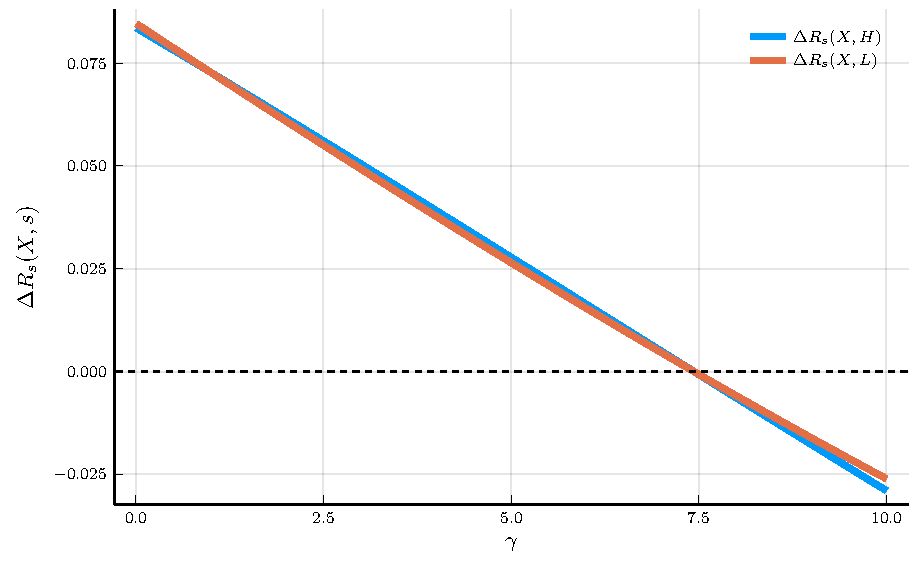
\includegraphics[width=0.8\textwidth]{figures/mehra_prescott.pdf}
    \caption{Mehra-Prescott limit}
    \label{fig:mehra_prescott}
	\caption*{\footnotesize
		Note: The solution is computed with the parameters $\beta = 0.99$,  $x_H = 1.018 + 0.036$, $x_L = 1.018 - 0.036$, $p_{HH} = p_{LL} =  (1+\rho)/2$, $\rho = 0.15$.
	}
\end{figure}

% \paragraph{Conclusion.} 
% In sum, we have seen that it is possible to have $\Delta R_{s}(X,H,L) < 0$ in equilibrium for some parameter values.
% Hence, we should not have assumed that the denominator is positive in the paper. 
% We have changed the expression in the paper to reflect this, as shown below:
% \changesbox{
%     \quoting{SDF}
% }







\commentbox{
\begin{enumerate}[start=2]
    \item I like Figures 4 and 5 a lot, but the numbers are crazy. Perhaps show the figures for
    EZ utility instead of IES=RA=1 so as to get something more ballpark?
\end{enumerate}
}

Thanks for this suggestion. We agree that, in the previous version, the numerical values
in Figures~\ref{fig: het_beliefs1} and~\ref{fig: het_beliefs2} were far from realistic, which could distract from the economic
mechanism the figures are meant to illustrate.

Because the purpose of these figures is to provide intuition within the analytically
transparent log-utility case, we retain the assumption of log utility. However, we have
recalibrated the model so that it matches standard asset-pricing moments more closely.
In particular, the revised calibration generates reasonable values for the Sharpe ratio,
which was notably off in the earlier version.

This adjustment preserves the simplicity of the log-utility environment while ensuring
that the numerical magnitudes shown in the figures are more in line with empirical
benchmarks.


\commentbox{
\begin{enumerate}[start=3]
    \item The data in table 3 is taken from three different papers – with in some cases
    mutually exclusive samples! This is not serious. It won’t change anything, but you
    should do a better job of choosing a sample and measuring yourself these easily
    available variables.
\end{enumerate}
}



We agree. In the previous submission, the data column in the (then) Table~3 relied on moments reported in multiple papers with different (and in some cases mutually exclusive) samples. In the revised paper, we now compute \emph{all} data moments from scratch using a single, transparent set of sources and clearly stated sample windows. In particular, we construct interest rates, excess returns, and dividend growth from the Shiller historical market dataset; consumption growth from BEA/FRED nondurables-and-services consumption per capita; and hours volatility from CPS series accessed via the BLS API (see the Data Appendix, Section~\ref{app:data_table5_moments}). 


In addition, beyond point estimates, we now quantify sampling uncertainty by computing moving-block bootstrap standard errors (and corresponding $\pm 2$ s.e.\ intervals) for each moment, and we report these intervals directly in the updated Table~\ref{tab:uncond_moments} (formerly Table~3). Details of the bootstrap procedure are described in the Supplementary Appendix (Data Appendix, Section~\ref{app:data_table5_moments}).

\commentbox{
\begin{enumerate}[start=4]
    \item Table 3 would benefit from clear column names.
\end{enumerate}
}

We thank you for this suggestion. In the revised paper, we have added clear column labels: ``Endowment'' (column 1, the endowment limit), ``Production'' (column 2, the production economy with labor friction), ``Homogeneous'' and ``Heterogeneous'' (columns 3--4, subjective beliefs without and with heterogeneity), ``High elast.'' (column 5, higher labor supply elasticity), and ``Data'' (column 6). We also expand the table notes to describe the exact specification considered in each column. 

\commentbox{
\begin{enumerate}[start=5]
    \item  I am not sure if the label of “diagnostic expectations” (DE) is correct for your
    Markov chain assumption. That's because DE, as you describe them, rely on an overreaction of beliefs to a shock. But suppose that in your setup, the Markov state
    does not change. That's a shock --- the realization of TFP growth differs from its
    conditional expectation --- but it does not affect beliefs. For this reason, I am not
    sure that I would call this DE or even extrapolative. It seems to me more precise to
    describe the setup as capturing different biases in beliefs across consumers, both
    their average belief bias and how the bias depends on the aggregate state.
\end{enumerate}
}

\medskip

Thank you for this thoughtful comment. We agree that the interpretation of
\emph{diagnostic expectations} depends critically on what is taken to be the relevant
\emph{reference group}, and that this distinction is especially salient when comparing
discrete-state and continuous-state environments. Our view is that the label
\emph{diagnostic expectations} is appropriate for our Markov-chain setup under the
natural choice of reference group in that context. Below, we clarify this interpretation
and explain why it differs from the continuous-state case that motivates your intuition.

\paragraph{Diagnostic expectations.}
Following \citet{GS10}, the \emph{representativeness} of a trait $T=t$ for group $G$
relative to a reference group $-G$ is defined as
\begin{equation}
R(t,G,-G) \equiv \frac{\Pr(T=t \mid G)}{\Pr(T=t \mid -G)}.
\end{equation}
A trait is said to be \emph{diagnostic} of a group if it is more representative of that
group than of the reference group.

As in \citet{bordalo2016stereotypes}, agents distort objective probabilities according to
\begin{equation}
Pr^i(T=t \mid G)
=
\frac{\Pr(T=t \mid G)\, h^i\!\big(R(t,G,-G)\big)}
{\sum_{t' \in \mathcal{T}} \Pr(T=t' \mid G)\, h^i\!\big(R(t',G,-G)\big)},
\end{equation}
where $h^i(\cdot)$ is a weighting function. We refer to expectations formed under this
distorted probability as \emph{diagnostic expectations}.

A commonly used specification is $h^i(R)=R^{\theta_i}$, yielding
\begin{equation}
Pr^i(T=t \mid G)
=
\underbrace{\Pr(T=t \mid G)}_{\text{rational beliefs}}
\times
\underbrace{\left(\frac{\Pr(T=t \mid G)}{\Pr(T=t \mid -G)}\right)^{\theta_i}}_{\text{belief distortion}}
\times C,
\end{equation}
where $C$ is a normalizing constant.

\paragraph{Diagnostic expectations in a Markov-chain environment.}
In our model, this structure maps naturally to a discrete-state Markov process. In
particular, the trait $T$ corresponds to next period's state $s_{t+1}$, the group $G$
corresponds to the current state $s_t=s$, and the reference group $-G$ corresponds to the
alternative state $s_t=-s$. Under this mapping,
\begin{equation}
\Pr^i(s_{t+1}=s' \mid s_t=s)
=
p_{ss'}
\left(\frac{p_{ss'}}{p_{-s s'}}\right)^{\theta_i}
\times C,
\end{equation}
which coincides with the belief distortion used in the paper.

If productivity growth is persistent under rational beliefs (i.e.,
$p_{HH}>p_{LH}$ and $p_{LL}>p_{HL}$), diagnostic expectations imply that agents overweight
state persistence: conditional on being in a high (low) state, remaining in that state is
perceived as especially representative. In this sense, agents overreact to the current
state, which is the discrete-state analogue of extrapolation.

\paragraph{Why this differs from the continuous-state intuition.}
Your interpretation applies more directly to continuous-state processes, where a shock
can be defined as a realization that differs from the conditional mean. In that setting,
diagnostic expectations typically require specifying a reference group such as the
expected value based on prior information.

For example, \citet{bordalo2020overreaction} consider an AR(1) process,
\begin{equation}
x_{t+1} = \rho x_t + \sigma \varepsilon_{t+1},
\end{equation}
and define the reference group using the conditional expectation $\rho x_{t-1}$ before $x_t$ is realized. The
distorted density then compares likelihoods relative to this benchmark, generating
overreaction to unexpected realizations.

In contrast, with a binary Markov chain, there is a natural reference
group---the alternative state. As a result, belief distortions operate through
state-dependent representativeness rather than through deviations from a conditional
mean. This explains why beliefs do not change following a realization that does not
trigger a state transition: representativeness is defined at the level of states, not
innovations.

\paragraph{Conclusion.}
In sum, our use of the term \emph{diagnostic expectations} is consistent with the formal
definition in the literature once the appropriate reference group is specified for a
discrete-state environment. Intuitively, when productivity is persistent, the current
state becomes especially representative under diagnostic beliefs, leading agents to
overestimate persistence. This mechanism is closely related to extrapolation, though
implemented differently than in continuous-state models.

To avoid confusion, we have added a clarifying footnote in the paper explicitly discussing
how our definition maps into standard formulations of diagnostic expectations, as shown below:
\changesbox{
    \quoting{DE_definition}
}
Of course, if you or the editor still feel that the terminology risks confusion, we would be
happy to adopt alternative wording.



\subsection*{Minor comments II}

\commentbox{
\begin{enumerate}[start=1]
\item As explained above, I think the use of LDF is confusing rather than its more logical
name, expected productivity growth under $Q$.
\end{enumerate}
}

Thank you for this suggestion. In the revised paper, we have removed the term ``LDF''
entirely and consistently use \emph{risk-neutral productivity growth} throughout. We
agree that this terminology is more natural and transparent, and it clarifies the
economic interpretation of the object as an expectation under the risk-neutral measure.

\commentbox{
\begin{enumerate}[start=2]
    \item Footnote 19 is quite obscure.
\end{enumerate}
}
To avoid any confusion, we decided to remove the footnote.

\commentbox{
\begin{enumerate}[start=3]
    \item Some of the authors’ language is a little peculiar. I am pretty sure that
    “intrapolation” is not widely used. (Googling it brings you directly to their paper…)
    What does it mean? “Interpolation”? Even that is not clear. It is worth defining what
    you mean by that (or even perhaps finding a more common term that captures the
    behavior you model).
\end{enumerate}
}

We thank you for this comment and agree. The term ``intrapolative" is not standard
and may cause confusion. In the revision, we replace it with \textit{contrarian beliefs}, which
more transparently captures the behavior we model ---agents who expect reversals rather
than persistence and are pessimistic in booms but optimistic in downturns. We believe
this terminology is more consistent with the asset-pricing and expectations literature.

\commentbox{
\begin{enumerate}[start=4]
    \item Similarly, the paper oscillates between “operational leverage” and “operating
    leverage”; I think the latter is more widely used.
\end{enumerate}
}

Thank you for pointing out this typo. We have replaced ``operational leverage'' with ``operating leverage'' throughout the paper.


\commentbox{
\begin{enumerate}[start=5]
    \item I find the citation of Sargent at the end a little cringe – what value does the cite
    add. But up to you of course.
\end{enumerate}
}

Thank you for this comment. If you are comfortable with it, we would like to keep the citation. We view the Sargent citation as adding useful context: it highlights the motivation for departing from full-information rational expectations, from a leading scholar of the rational expectations revolution. Of course, if you prefer, we are happy to remove the citation.

\commentbox{
\begin{enumerate}[start=6]
    \item Succesfully typo in conclusion
\end{enumerate}
}

Fixed.

\commentbox{
\begin{enumerate}[start=7]
    \item We “define” no p12 – it’s already defined.
\end{enumerate}
}

In the revised version of the paper, we do not discuss the human wealth at this point anymore, so this phrase has been removed. 

\commentbox{
\begin{enumerate}[start=8]
    \item Ci0t tilde in eqn 9 p13? Why not just Ci tilde?
\end{enumerate}
}

Fixed.

\commentbox{
\begin{enumerate}[start=9]
\item I kept getting confused with the subscripts $r,e$ in returns (and I think the authors
themselves get confused --- see $j\in\{r,b\}$ after equation (11)). Why not use simpler
notation, such as $R_s$ for stock returns and $R_x$ for excess returns?
\end{enumerate}
}

As discussed in our response to your second major
comment, we have substantially simplified the notation in the revised paper by focusing
on the case of linear labor disutility ($\nu=0$). This special case preserves the main
economic mechanisms while allowing for a much more transparent exposition.

In the revised version, there is a single risky asset (stocks). We denote its gross return
by $R_{r,t}$ and its excess return by $R_{r,t}^e \equiv R_{r,t}/R_{f,t}-1$, which follows
standard asset-pricing notation (see, e.g., \citealt{cochrane2005asset}). The additional
return objects present in the previous version have been eliminated, and we have checked
that the notation is now used consistently throughout the paper.

We hope this change resolves the confusion regarding return notation.


\commentbox{
\begin{enumerate}[start=10]
    \item ``attenuate the subsequent decline in TFP growth" - I think you mean, attenuate
    the effects of the subsequent decline in TFP growth
\end{enumerate}
}

Fixed.


% Test reference to paper: You can reference sections like Section~\ref{sec:conclusion} 
% or equations like Equation~\ref{eq:realized_earnings} from the main paper.

% Add your response to Reviewer 1 here



% \newpage

% \input{Letters/Letter_R2.tex}

% \newpage

% \input{Letters/Letter_R3.tex}

% \singlespace
\newpage
\bibliography{../../../../utils/references/references.bib,../../../../utils/references/references_empirical.bib}

\end{document}

